\documentclass[sigplan,10pt]{acmart}

\settopmatter{printacmref=false}
\renewcommand\footnotetextcopyrightpermission[1]{}
\pagestyle{plain}
\settopmatter{printfolios=true}

\graphicspath{{../figures/}{figures/}}
\usepackage[utf8]{inputenc} % allow utf-8 input
\usepackage[T1]{fontenc}    % use 8-bit T1 fonts
\usepackage{hyperref}       % hyperlinks
\usepackage{url}            % simple URL typesetting
\usepackage{booktabs}       % professional-quality tables
\usepackage{amsfonts}       % blackboard math symbols
\usepackage{nicefrac}       % compact symbols for 1/2, etc.
\usepackage{microtype}      % microtypography
\usepackage{xcolor}         % colors
\usepackage{graphicx}
\usepackage{stfloats}
\usepackage{xspace}
\usepackage{multirow}
\usepackage{tikz}
\usetikzlibrary{arrows.meta,positioning}
\usepackage{comment}
\usepackage{enumitem}
\usepackage{algorithm}
\usepackage{algpseudocode}

\usepackage{pifont}
\newcommand{\cmark}{\ding{51}}
\newcommand{\xmark}{\ding{55}}
\newcommand{\zl}[1]{{\color{red}{#1}}}
\newcommand{\wzw}[2]{{\color{blue}{#2}}}

\hypersetup{colorlinks=true,linkcolor=black,citecolor=black,urlcolor=black}

% Observation callout box
\newcommand{\observation}[1]{%
  \smallskip\noindent\fbox{\parbox{0.96\columnwidth}{%
    \small\textbf{Observation.}~#1}}\smallskip}

\newcommand{\sysname}{OmniFlow\xspace}
\def\task-nums{30}

\title{\sysname: Adaptive On-device Replay System for Mobile GUI Agents}

\begin{document}

\begin{abstract}
    abs
Modern mobile UIs change between users, devices, and sessions: layouts
re-flow, stable selectors are often absent, and content is personalized.
LLM-based GUI agents handle this dynamism by re-reasoning at every
step---effective on open-ended tasks, but expensive on the recurring
routines that dominate real device use.  Each step in their reason-act
loop may require a fresh model decision, incurring on-device latency,
memory, power, and thermal cost, or expanding the privacy boundary when
screens are shipped to a cloud planner.  Trajectory reuse is the natural
serving target, but existing record-and-replay, memory-retrieval, and
program-guided systems still fall back to online repair the moment
those same dynamic conditions invalidate a stored action.

We present \textbf{OmniFlow}, a plug-in cache for mobile GUI agents
whose central design is to \emph{check and remap every recalled action
against the live screen before it executes}, so historical executions
become reusable Functions without requiring identical layouts, selectors,
or coordinates at reuse time.  \wzw{}{\textbf{Omni} writes successful
run logs into a Function Store whose assets are API-like
\texttt{Functions}; the store induces sparse UDEG nodes as a
privacy-safe state index that keeps raw XML, screenshots, and personal
text outside the shared cache boundary.}
\wzw{}{Recall returns compact executable candidates rather than full trajectories.}
\textbf{Flow} drives a recalled Function on the live device through an
observe-check-transfer-act loop that checks each action against the current
state, remaps the target, executes when safe, and falls back otherwise.  Matched Functions therefore skip
online reasoning entirely, while uncertain states remain under the host
agent through a structured handoff.

On androidworld benchmarks, OmniFlow enables 2.3$\times$ reuse of successful trajectories, improving task success rates by 5.4\% and reducing latency by 25\% on average, with up to 40\% improvement on challenging dynamic tasks.  User studies show that OmniFlow's reuse leads to smoother interactions and higher satisfaction, especially on tasks with dynamic content.  By enabling robust trajectory reuse, OmniFlow significantly enhances the efficiency and user experience of LLM-based GUI agents in the face of mobile UI dynamism.

\end{abstract}

\maketitle
\section{Introduction}
\label{sec:intro}

% Mobile GUI agents powered by vision-language models (VLMs) are commonly designed for open-ended task execution.
% At each step, the agent observes the current screen, invokes a model to decide the next action, executes one GUI operation, and repeats this loop until the task is complete.
% This design is effective for novel tasks because the agent can reason over arbitrary screens and user goals.
% However, it is an inefficient serving path for a large class of real mobile workloads: repeated GUI execution.

% In daily mobile use, many tasks recur with similar structure.
% Users repeatedly open the same app pages, search for similar content, fill similar forms, change common settings, confirm routine operations, and navigate through familiar workflows.
% For these recurring tasks, step-wise reasoning forces every user and every repetition to solve nearly the same interaction sequence again.
% This repeated model invocation introduces computation, memory, energy, and thermal overheads on edge devices.
% When the model is served in the cloud, it can also expose screenshots, view hierarchies, and private app content to an external planner.
% These costs motivate a different serving target for mobile GUI agents:
% \textit{successful execution histories should be reused whenever the current task and live environments are compatible.}

Mobile GUI agents powered by vision-language models (VLMs) have demonstrated impressive capabilities in open-ended task execution.
However, when deployed in the real world, users rarely utilize these agents solely for open-ended exploration.
Instead, users expect them to act as intelligent assistants that accelerate daily, repeated routines--such as checking schedules, filling out common forms, or navigating familiar app workflows--fast and reliably.
Currently, mobile GUI agents address these tasks using a standard observe-reason-act loop~\cite{abhyankar2025osworld,rawles2025androidworld,wen2024autodroid,wang2023enabling}: observing the current screen, invoking a massive model to decide the next action, executing the operation, and repeating until completion.
While this design is highly effective for novel tasks with the support of performant VLMs, applying step-wise VLM reasoning to recurring routines forces every user and every repetition to solve nearly the same interaction sequence from scratch.
This repeated model invocation introduces severe computation, memory, energy, and thermal overheads on edge devices.
This reality motivates a new serving target for mobile GUI agents:
\textit{successful execution histories of daily routines should be efficiently reused to bypass expensive model invocations whenever possible.}

Existing systems have attempted to address this serving target through various approaches, as summarized in Table~\ref{tab:comparison}. 
(1) Per-step acceleration methods~\cite{chen2025less,dai2025advancing,lin2025showui,gomez2013reran} reduce the latency of individual model calls but fail to break the expensive observe-reason-act loop.
(2) Traditional RPA-style replay and script-based tools~\cite{li2017sugilite,gomez2013reran,maestro2026,openatx_uiautomator2_2026} eliminate model calls by binding execution to fixed coordinates or fixed UI selectors, yet they are highly brittle to GUI dynamics.
(3) Meanwhile, memory-based agents~\cite{wen2024autodroid,zhang2025appagent,lee2024mobilegpt} retrieve prior task knowledge but still require online VLM reinterpretation, leaving them too heavy for seamless on-device execution.

Crucially, these prior studies fall short because they cannot accommodate the complex realities of real-world mobile environments, which are driven by two fundamental dynamics.
First, \textbf{workflow-level dynamics} mean that live tasks frequently diverge from recorded trajectories due to unpredictable interruptions like login screens, pop-up ads, loading delays, or alternative app entry points.
A rigid script fails entirely when the exact path breaks.
Second, \textbf{GUI-state-level dynamics} dictate that even when the overall workflow aligns, the concrete target on the screen may shift due to different device resolutions, font scales, dynamic content, or app updates.
Existing approaches mismatch this reality: they are either too expensive by re-planning every step, or too brittle by blindly replaying actions without adapting to shifting GUI states.

To this end, we propose \textsc{OmniFlow}, an adaptive on-device replay system for mobile GUI agents.
OmniFlow is designed to seamlessly reuse historical execution fragments while gracefully falling back to VLM reasoning when necessary.
The system is built around two core components:
(1) the Omni representation layer, which decomposes past executions into a fine-grained UI transition graph of reusable functions, and
(2) the Flow execution layer, which dynamically grounds and verifies recalled actions into the live GUI state before execution.


These two components are specifically designed to solve the aforementioned dynamics through two core technical innovations.
First, to tackle workflow dynamics and efficiency, OmniFlow employs a fine-grained transition graph coupled with a fast on-device node matching mechanism.
Unlike prior memory systems that rely on computation-heavy visual embeddings, OmniFlow's node encoding relies entirely on feature-engineered page vectors derived from the accessibility-tree structure.
This allows for rapid, lightweight node matching executed completely on the mobile device.
By matching fine-grained UI states rather than monolithic trajectories, OmniFlow can smoothly alternate between trajectory reuse and VLM reasoning.
This maximizes the utilization of stored memories: if a workflow diverges due to a pop-up ad, the system falls back to the VLM to clear it, and instantly resumes replay-based execution once a recognized GUI state is reached.

Second, to address GUI-state dynamics, OmniFlow introduces an anchor-based action transfer design within the Flow execution layer.
Instead of executing actions via static coordinates, this mechanism grounds a recorded action in the live GUI by comparing structural, visual, and geometric features between the recorded state and the current screen.
It identifies stable neighboring elements as anchors and uses local layout relations and GUI-tree structures to dynamically locate the intended target.
If the target match lacks confidence or is blocked by runtime conditions, the system abstains and defers to VLM generation, ensuring robust adaptation to shifting layouts and device variations.

We implement OmniFlow as a plug-in cache and execution layer integrated into mobile GUI agents.
We evaluate OmniFlow on the AndroidWorld benchmark, comparing it against \zl{xxx} baselines.
Our experimental results demonstrate that \zl{yyy}.

% Existing systems only partially address this target, as we summarized in Table~\ref{tab:comparison}.
% Step-wise GUI agents improve action generation or verification, but still invoke a model for each interaction.
% (1) Per-step acceleration methods~\cite{chen2025less,dai2025advancing,lin2025showui,gomez2013reran} reduce the cost of each model call, while retaining the same observe-reason-act loop.
% (2) RPA-style replay and script-based systems avoid model calls, but bind execution to a fixed trajectory, coordinate sequence, selector set, or app state~\cite{li2017sugilite,gomez2013reran,maestro2026,openatx_uiautomator2_2026}.
% (3) Memory-based agents~\cite{wen2024autodroid,zhang2025appagent,lee2024mobilegpt} retrieve prior task knowledge or UI transition graphs, but the retrieved memory often requires online reinterpretation and provides limited support for execution under dynamic layouts, devices, users, and app versions.
% As a result, existing approaches mismatch the repeated-execution workload: they either remain too expensive by re-planning for every step, or become too brittle by replaying stored actions without sufficient adaptation.

% We revisit the objective of repeated mobile GUI execution.
% For recurring tasks, the system does not need to reproduce an entire historical trajectory, nor does it need to re-invoke the VLM for every step.
% Instead, it should preserve and re-execute the task effect of reusable interaction fragments.
% For example, a prior execution that opens a search page, enters a query, selects a result, or confirms a form should become a callable operation that can be reused in later tasks.
% This objective requires adaptive replay: the system must decide when a historical operation is applicable, transfer it to the current GUI state, execute it safely, and fall back to the underlying GUI agent when reuse is uncertain.

% Adaptive replay is difficult because mobile GUI execution is dynamic at two levels.
% First, repeated tasks exhibit workflow-level dynamics.
% A live task may diverge from a recorded path because of login state, permission dialogs, advertisements, pop-ups, loading delays, personalized content, or alternative app entry points.
% A complete recorded trace may no longer match the live workflow, even though many of its local fragments remain useful.
% Second, mobile apps exhibit GUI-state-level dynamics.
% Even when the current screen corresponds to a memorized state, the concrete action target may shift because of device size, density, font scale, orientation, app version, language, user content, or missing accessibility attributes.
% Thus, a useful replay system must support both partial workflow reuse and state-aware action transfer.

% We present \textsc{OmniFlow}, an adaptive replay system for mobile GUI agents.
% \textsc{OmniFlow} wraps an existing agent-device loop with a cache-first execution layer.
% When a compatible reusable operation is found, \textsc{OmniFlow} executes it directly without invoking the VLM for the matched steps.
% When the memory is missing, unsafe, or ambiguous, \textsc{OmniFlow} returns control to the original GUI agent.
% This design preserves the open-ended capability of step-wise agents while amortizing the cost of recurring GUI workflows.

% \textsc{OmniFlow} is built around two components.
% The first is the \emph{Omni representation layer}, which converts successful run logs into reusable execution knowledge.
% Instead of storing a whole task as a monolithic trajectory, Omni decomposes executions into UDEG nodes and callable Functions.
% A UDEG node represents an action-compatible GUI state cluster, while a Function represents a task-carrying transition with a start condition, argument schema, action sequence, and compact execution evidence.
% This granularity allows the system to reuse matched fragments of a historical execution, fall back to VLM reasoning when the live workflow diverges, and resume memory-guided execution when another compatible state is reached.

% The second component is the \emph{Flow execution layer}, which applies recalled Functions to the live device state.
% Flow executes each Function through an observe-check-transfer-act loop.
% Before dispatching a cached action, Flow observes the current screen, checks whether the pending operation is safe, transfers the recorded target to the live GUI, and executes only when the target is sufficiently confident.
% To support this transfer, Flow uses anchor-based action grounding.
% It matches stable source-current GUI elements as anchors, projects the recorded target through these anchors, and selects the live target using element similarity, local geometry, and UI-tree relations.
% If the evidence is weak or ambiguous, Flow abstains and falls back to recovery or VLM-based action generation.

% \textsc{OmniFlow} builds on two cooperating components.  The first component, Omni representation layer, organizes past executions into reusable execution fragments.
% A successful run is decomposed into compact state descriptions and callable Functions, where each Function captures a task-relevant operation, such as opening a search page, entering a query, selecting an item, or confirming a form.
% Each Function is associated with the state condition under which it can be applied, the arguments that should be rebound at runtime, and the action sequence needed to produce the intended task effect.
% This representation gives the system a finer-grained reuse unit than a full historical trajectory.
% During a live task, Omni representation layer can recall a Function from any compatible intermediate state, execute the reusable fragment, and return control to the underlying GUI agent when the current workflow moves outside the recalled context.
% If the execution later reaches another compatible state, reuse can resume from that point.
% In this way, the memory layer makes replay less dependent on the live task following the same end-to-end path as the original execution.

% The second component, Flow execution layer, grounds each recalled Function in the current GUI before execution.
% A recalled Function describes what operation was useful in the past, while the live screen determines whether and how that operation can be executed now.
% Therefore, it runs each cached action through an observe-check-transfer-act loop.
% It observes the current screen, checks whether the pending action is valid under the live state, maps the recorded target to a current GUI element, and dispatches the action only when the match is sufficiently confident.
% For target mapping, Flow uses anchor-based transfer.
% It compares the recorded screen and the live screen through element-level visual, structural, geometric, and interaction features, then uses stable neighboring elements as anchors to locate the current target.
% The final target is selected using local layout relations, tree structure, element compatibility, and confidence-margin checks.
% When the evidence is weak, ambiguous, or blocked by runtime conditions such as dialogs or advertisements, Flow abstains and hands control back to recovery logic or VLM-based action generation.

% Together, these mechanisms make adaptive replay possible under dynamic mobile execution.
% The Omni representation layer increases the chance that useful parts of a prior execution can still be reused after workflow divergence.
% The Flow execution layer checks and transfers each recalled action against the live screen before it is performed.
% This separation lets \textsc{OmniFlow} exploit repeated structure in mobile tasks while preserving the underlying GUI agent as the fallback path for novel, unsafe, or semantically ambiguous states.

% We implement \textsc{OmniFlow} as a plug-in cache and execution layer for Android GUI agents.
% \zl{
% Our current evaluation shows that \textsc{OmniFlow} can convert successful prior executions into zero-model-call Function replay on matched tasks, while retaining fallback for uncertain states.
% On the accepted AndroidWorld replay set, \textsc{OmniFlow} completes all \task-nums validator-scored reuse runs with zero online model calls and zero online model tokens.
% For cross-device UDEG retrieval, \textsc{OmniFlow} achieves 98.63\% Hit@1 and 100.0\% Hit@3 on the currently reviewed subset, with sub-millisecond lookup latency.
% These results suggest that adaptive replay is a practical complement to VLM-based GUI agents: step-wise reasoning handles novel or ambiguous states, while \textsc{OmniFlow} serves recurring GUI fragments through verified reusable Functions.
% }

This paper makes the following contributions.

\begin{itemize}
    \item We identify repeated mobile GUI execution as a critical real-world serving workload for VLM-powered GUI agents, and formally characterize the workflow-level and GUI-state-level dynamics that render existing replay-based methods insufficient.
    \item We design \textsc{OmniFlow}, an adaptive on-device replay system that overcomes mobile GUI dynamics through two cooperating mechanisms: fast on-device node matching on fine-grained execution trajectories to seamlessly alternate between memory reuse and VLM reasoning, and anchor-based action transfer to robustly execute recorded actions on live screens.
    \item We implement and evaluate OmniFlow on several mobile GUI agents and representative benchmarks. Results show that \zl{xxx}.
    % \item We design \textsc{OmniFlow}, an adaptive on-device replay system that leverages a fine-grained UI transition graph and fast on-device node matching to seamlessly alternate between trajectory reuse and VLM reasoning.
    % \item We implement and evaluate \textsc{OmniFlow} on repeated mobile GUI tasks, showing that reusable Functions can reduce online model invocation cost while preserving fallback to the underlying GUI agent.
    % \item OmniFlow's replay path requires no VLM and no embedding model: state matching and action transfer rely entirely on feature-engineered page vectors derived from accessibility-tree structure, so the full reuse pipeline runs on mobile CPU hardware with zero online model tokens on a cache hit, retaining only a lightweight chat LLM for cache-miss fallback.
\end{itemize}

\section{Background and Motivation}
\label{sec:background}
\label{sec:motivation}

In this section, we review recent advances in mobile GUI agents powered by emerging LLMs and VLMs, along with the high execution costs associated with the traditional execution pipeline.
We then examine efforts to reduce the runtime costs of such agents and discuss their limitations, which motivate the design of \sysname.

\begin{figure}[t]
  \centering
  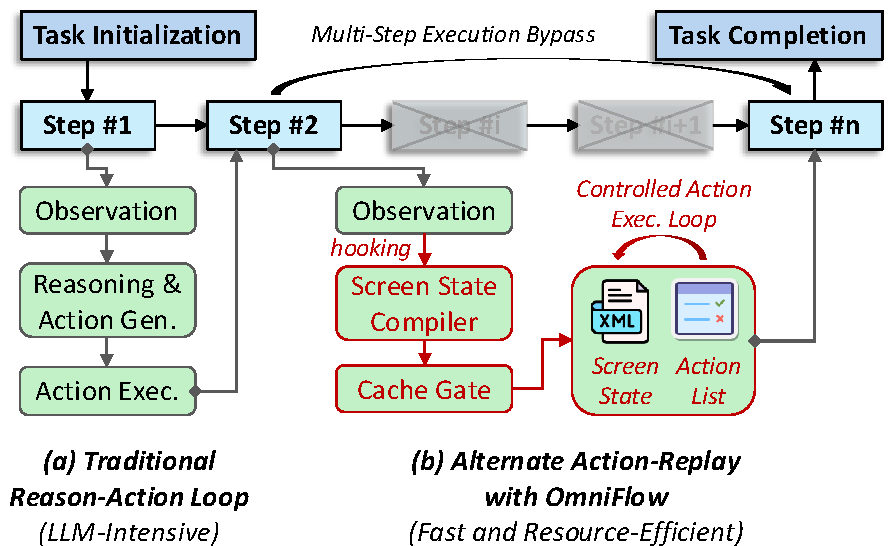
\includegraphics[width=0.45\textwidth]{figs/F14_comparison.pdf}
  \caption{Overview of \sysname workflow.
  The framework dynamically alternates between a traditional LLM-intensive reason-action loop (a) and a fast action-replay mechanism (b) to accelerate task execution.
  By hooking observations and querying the memory, the system recognizes familiar screen states and adaptively replays a cached list of atomic actions.}
  \label{fig:intro-comparison}
\end{figure}

\subsection{High Execution Costs of GUI Agents}
\label{sec:obs1}
\label{sec:obs2}

Mobile GUI agents typically operate in an observe--reason--act loop~\cite{rawles2025androidworld,wen2024autodroid,zhang2025appagent,wang2023enabling}.
As shown in Figure~\ref{fig:intro-comparison}, at each step, the agent perceives the current screen, invokes an LLM or VLM to determine the next GUI action, and executes the action in the environment.
Although this workflow enables flexible reasoning over open-ended tasks, it introduces substantial runtime overhead because model inference is repeatedly triggered during long interaction sequences.
The cost accumulates with each additional step, leading to increased latency and computation during task execution~\cite{dai2025advancing,zhang2025does,abhyankar2025osworld,zhong2026actionengine,zhang2025ufo2}.
Prior work reports that existing mobile agents often require more than 10 seconds per step, 1--2 minutes, and about \$1 monetary cost per task on average~\cite{dai2025advancing,christianos2025lightweight}.
More broadly, planning and reflection alone can account for 75\%--94\% of end-to-end latency in GUI agents~\cite{abhyankar2025osworld}.
These costs become more pronounced when the step-wise model inference runs directly on mobile devices with strict memory, power, and thermal constraints~\cite{dai2025advancing,christianos2025lightweight,zhang2024large}.

However, real-world mobile usage rarely consists of purely open-ended tasks.
In practice, users repeatedly perform similar routines, such as checking routine information, retrieving specific content, completing fixed navigation paths, and filling structured form-like workflows.
Prior studies characterize smartphone interaction as highly habitual, with repetitive checking behavior and app-launch patterns that are strongly shaped by recurring contexts such as time and location~\cite{oulasvirta2012habits,yan2012fast}.
Public mobile GUI datasets and benchmarks also reflect a similar pattern.
For example, the largest scale mobile GUI dataset to date, AITW, contains 715K episodes but only around 30K unique instructions~\cite{rawles2023android}.
We further quantify recurrence over the 30,378 subset-level unique-prompt entries reported across AITW's five subsets (Appendix~\ref{app:aitw-prompt-similarity}).  Parameter masking alone finds a template peer for 11,052 prompts (36.4\%).  Under a conservative criterion that accepts either a shared parameter template or semantic similarity of at least 0.98 while rejecting opposite intents, 22,834 prompts (75.2\%) have at least one similar counterpart; lowering the semantic threshold to 0.95 raises the estimate to 86.9\%.  These prompt-level rates estimate the workload available to a Function cache: they characterize candidate reuse demand, while executable Function reuse additionally requires compatible GUI state, action transfer, and terminal-effect verification.
Therefore, although per-step reasoning for open-ended tasks is crucial for high task completion rates, many realistic mobile-agent workloads are better viewed as repeated executions of recurring workflow patterns.

\zl{[This paragraph is the limitations of existing replay mechanisms; it also introduces massive new concepts such as coordinate replay and selector replay, which have not been introduced ahead.]}
This reuse problem is constrained by the observation interface itself.
Mobile GUI agents usually observe a screenshot, an Android accessibility tree, or both.
The accessibility tree reliably exposes element bounds and hierarchy when elements are observable, while semantic attributes such as \texttt{resource-id}, \texttt{text}, and \texttt{content-desc} only appear when developers provide them.
As a result, repeated execution cannot assume that every target has a stable selector: coordinate replay breaks under device-size and layout changes, and selector replay fails on missing annotations, custom-rendered widgets, WebViews, obfuscated resource identifiers, and unlabeled container controls.
The same instability limits graph-level reuse.
A conventional UI transition graph provides a useful state structure, but its nodes are often tied to raw XML or unstable attributes, and its edges record dispatched actions and state transitions rather than verified task effects.
\wzw{}{The missing object is a callable transition: a UTG edge can record that one action once moved an app from one observed state to another, but it does not by itself package runtime arguments, source-context transfer, or terminal/effect verification as an API-like operation.}
Such a graph is therefore difficult to reuse as a cross-device and cross-user execution cache under dynamic layouts and user-specific content.

\begin{table}[t]
  \centering
  \caption{Execution acceleration methods for mobile GUI agents.
  The columns capture whether a method (1) requires prior exploration on GUI states, (2) utilizes a cached memory without
  invoking LLM/VLM again, and (3) transfers its memory to dynamic and heterogeneous execution environments.}
  \label{tab:comparison}
  \resizebox{\columnwidth}{!}{
  \begin{tabular}{@{}lccc@{}}
  \toprule
  \textbf{Method}
    & \textbf{\begin{tabular}[c]{@{}c@{}}W/ App\\Exploration\end{tabular}}
    & \textbf{\begin{tabular}[c]{@{}c@{}}W/ Model\\Invocation\end{tabular}}
    & \textbf{\begin{tabular}[c]{@{}c@{}}Cross-Env\\Transferability\end{tabular}} \\
  \midrule
  RPA/script replay~\cite{li2017sugilite,gomez2013reran,maestro2026,openatx_uiautomator2_2026}
    & \cmark & \xmark & \xmark \\
  Memory-based~\cite{wen2024autodroid,zhang2025appagent,lee2024mobilegpt}
    & \cmark & \cmark & \xmark \\
  Program-guided~\cite{autodroid-v2,zhong2026actionengine,wang2026imperative,tian2025agentprog}
    & \cmark & \xmark & \xmark \\
  Per-step acceleration~\cite{dai2025advancing,lin2025showui,chen2025less,ouyang2026focusui}
    & \xmark & \cmark & \xmark \\ \hline
  \textbf{\sysname}
    & \textbf{\xmark} & \textbf{\xmark} & \textbf{\cmark} \\
  \bottomrule
  \end{tabular}
  }
\end{table}


\subsection{Reducing Runtime Costs}
\label{sec:bg-replay}
\label{sec:bg-programmatic}
\label{sec:bg-utg}

Prior studies on reducing the runtime costs of GUI agents primarily fall into several categories, which are summarized in Table~\ref{tab:comparison}.

\textbf{Robotic process automation (RPA)-based automation systems} treat mobile tasks as fixed workflows by recording and replaying user demonstrations~\cite{li2017sugilite,gomez2013reran,maestro2026,openatx_uiautomator2_2026}.
These systems construct replayable execution traces through human-driven app exploration before task execution.
However, the resulting memory is tightly bound to the recorded execution path, GUI layout, and entry state.
As a result, even minor changes in the live GUI state, such as screen modifications or layout updates, can cause the recorded execution to fail.

\textbf{Memory-based GUI agents} reduce runtime costs by reusing memory constructed from prior app exploration or first-time task execution.
For example, M3A~\cite{rawles2025androidworld} stores prior actions and their reasoning in prompts to guide later execution.
AutoDroid~\cite{wen2024autodroid} and AppAgent~\cite{zhang2025appagent} construct app-specific memory, such as UI transition graphs, through automated exploration and retrieve this memory during execution.
MobileGPT~\cite{lee2024mobilegpt} extends this idea with hierarchical app memory that stores reusable procedures and subtasks summarized from prior executions.
MobiMem~\cite{liu2025beyond} reduces repeated GUI-agent reasoning by reusing prior executions through experience memory, which abstracts task traces into reusable templates, and action memory, which caches low-level action sequences for direct replay.
\textbf{Program-guided agents}~\cite{autodroid-v2,zhong2026actionengine,wang2026imperative,tian2025agentprog} further reduce runtime costs by translating task knowledge or prior demonstrations into executable scripts.
These scripts allow repeated GUI operations to be completed through deterministic program execution with fewer model invocations.
Together, memory-based and program-guided agents replace parts of VLM-based step-wise action generation with previously validated memory or executable operations.
However, these methods still rely on memory constructed from prior app exploration, user interaction, or first-time execution, which can introduce privacy concerns and limit transfer across users, devices, app versions, and unseen environments.

% Related memory mechanisms have also been explored in AppAgentX, which identifies repetitive action sequences from execution history and compiles them into higher-level shortcuts~\cite{jiang2025appagentx}.
% \zl{AxNav~\cite{taeb2023axnav}, UINav~\cite{li2023uinav}, AutoTask~\cite{pan2023autotask}}

% Third, \textbf{program-guided agents} generate executable scripts or programs
% from collected app documentation, state-machine memory, or declarative
% interfaces~\cite{autodroid-v2,zhong2026actionengine,wang2026imperative,tian2025agentprog}.
% These systems improve long-horizon control, but they still rely on substantial
% app knowledge and online adaptation when the live state diverges from the
% stored program.

Another line of studies, \textbf{per-step inference acceleration methods}, retain the traditional observe--reason--act loop while reducing the cost of each individual decision.
V-Droid~\cite{dai2025advancing} replaces auto-regressive action generation with verifier-based ranking over a discretized action space, which substantially reduces latency.
ShowUI~\cite{lin2025showui} accelerates VLM inference through UI-guided visual token selection.
Other studies accelerate execution by pruning redundant visual or historical context before model inference, such as masking-based GUI element pruning, history compression~\cite{chen2025less}, and position-preserving UI token selection~\cite{ouyang2026focusui}.

To summarize, existing approaches still face several limitations.
RPA-based systems and script replay provide executable workflows, but they are fragile when the live GUI state diverges from the recorded execution.
Memory-based and program-guided agents reduce repeated reasoning, but they often rely on substantial app exploration and provide limited support for workflow-level adaptation.
Per-step inference acceleration methods reduce the cost of each individual decision, but they still require repeated VLM-based step-wise action generation in long interaction loops.
These limitations motivate us to build \sysname for generalizable memory reuse across dynamic app environments.

\subsection{Goals and Challenges}
\label{sec:obs3}
\label{sec:obs-need}

Mobile apps dynamically change across users, devices, and sessions and often lack stable APIs for GUI agents to invoke. While traces usually expose a fixed-action subspace:
within a ReAct loop, recurring tasks often contain high-frequency repeated
Functions, such as opening a search page, entering a query, filling a form, or
confirming a save.  We call such reusable units \texttt{Functions}.  This
observation suggests storing them as persistent Functions that can be updated over
time, so the agent can skip reasoning and execute directly when the same
situation recurs.

Our goal is to design a memory system for mobile GUI agents that can reuse past executions in dynamic app environments while allowing flexible switching between memory-guided execution and VLM-based step-wise action generation.
This requires memory to support both workflow-level adaptation, where the execution path may change, and state-level adaptation, where a memorized GUI state may appear differently from the live GUI state.


\textbf{Adaptive Reuse Workflow.}
The first challenge is representing past executions at a granularity suitable for flexible reuse.
Existing memory systems for GUI agents often store a complete long-horizon trajectory or split it into fixed subtasks, then guide the agent to follow the recorded execution path.
This design is fragile in real mobile apps, where workflows frequently change due to expired login sessions, pop-ups, loading delays, or permission dialogs.
A coarse-grained memory may fail even when most parts of the historical execution remain reusable.
This calls for a finer-grained memory representation that can reuse matched Functions while allowing the agent to fall back to VLM-based step-wise action generation when the live workflow diverges.

\textbf{Adaptive Action Grounding.}
The second challenge is applying a memorized operation to a live GUI state safely.
Even when the live GUI state corresponds to a memorized GUI state, the target GUI component may shift due to screen size, font scale, list ordering, or dynamic content.
This requires the system to be able to utilize historical context to achieve localization enhancement.

\begin{table}[t]
  \centering
  \caption{Execution costs of different on-device inference backends.We use Qwen-vl-0.8B-W4A16 on OnePlus 12.}
  \label{tab:ondevice-cost}
  \resizebox{\columnwidth}{!}{%
  \begin{tabular}{llllr}
    \toprule
    Location & Backend & Input & Tokens & Time \\
    \midrule
    On-device & Llama.cpp & screenshot & $\sim$2,500 & 60\,s+ \\
    On-device & MNN-LMM  & screenshot & $\sim$2,500 & 10\,s+ \\
    Cloud     & Qwen-API  & screenshot & $\sim$3,200 & 3\,s  \\
    \bottomrule
  \end{tabular}}
\end{table}

% Design
% Requires in preamble: \usepackage{tikz}  \usetikzlibrary{arrows.meta,positioning}
\begin{figure*}[t]
  \centering
  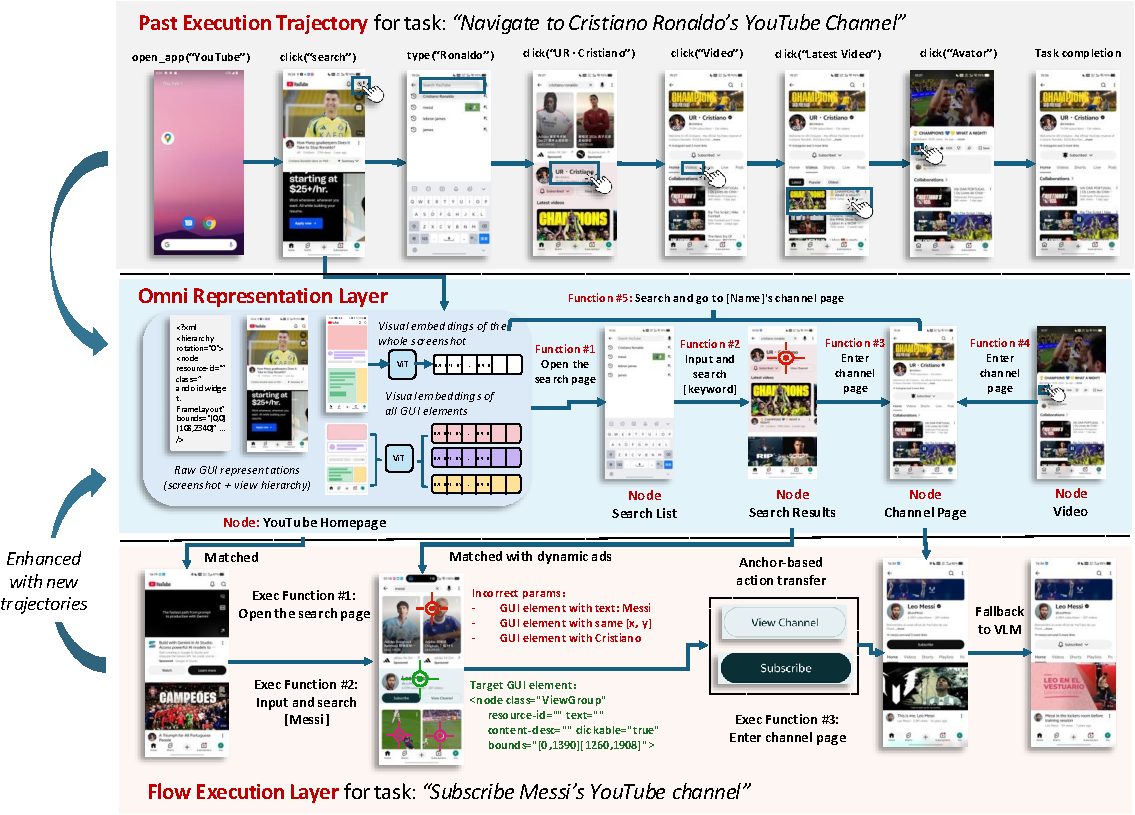
\includegraphics[width=0.94\textwidth]{figs/demo.pdf}
  \vspace{-0.5em}
  \caption{Demonstration of how a task execution trajectory is transformed into memory and how that memory is adaptively utilized in online execution environments.}
  \label{fig:demo}
  \vspace{-0.6em}
\end{figure*}

\begin{figure*}[t]
  \centering
  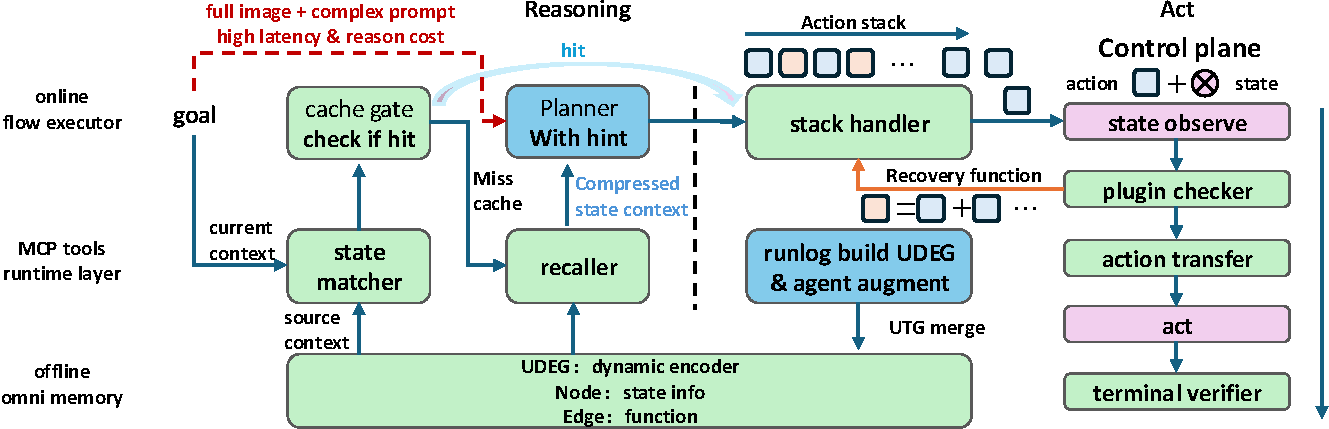
\includegraphics[width=0.94\textwidth]{figs/F20_system_design.pdf}
  \vspace{-0.5em}
  \caption{\wzw{}{System design overview.
  OmniFlow builds a Function Store whose assets are API-like Functions synthesized from successful GUI executions.
  The store induces a sparse UDEG: privacy-safe GUI-state nodes index where Functions can be invoked, and Function edges record executable task effects.
  \textsc{Omni} recalls a compatible Function through this state index; \textsc{Flow} executes it through a single observe-check-transfer-act stack and writes accepted run logs back into the Function Store.}}
  \label{fig:pptx-system-design-overview}
  \vspace{-0.6em}
\end{figure*}

\section{System Design}
\label{sec:design}

\subsection{Architecture and Workflow}
\label{sec:design-overview}

\sysname consists of two layers.
(1) \textsc{Omni} representation layer manages history traces and converts them into reusable and callable memory functions.
(2) \textsc{Flow} execution layer  executes recalled Functions and VLM-generated actions on the live device. 



% ───────────────────────────────────────────────────────────────────────────
\subsection{\textsc{Omni} Representation Layer}
\label{sec:design-offline}



\textsc{Omni} exposes two interfaces: \emph{recall} retrieves executable Functions from the Function Store, and \emph{Update} ingests execution logs into the Function Store for offline enhancement.

\textbf{UDEG.} \sysname builds a UDEG (Universal-Device-Execution Graph) to support cross-device and cross-user Function reuse. UDEG nodes are clusters of GUI states, and edges are executable Functions.

Some works use UTG (UI transition graph) to represent the app state space, but mobile GUI states are often highly dynamic and user-specific, which makes UTG need to be updated frequently. Instead of storing raw screenshots or raw XML, UDEG nodes store compact feature vectors that capture the visual, structural, geometric, and interaction cues of the GUI state. \sysname uses xml-feature compactor to acomplish page embedding because vision-embedding-model is expensive and privacy-sensitive, while xml features are cheap and structured. We prove in \S\ref{sec:evaluation} that this representation is sufficient for high-accuracy page matching and Function recall.

For each element, it builds a 64-dimensional feature vector from two sources:
screenshot-derived visual cues, such as icons, labels, and clickable regions, and view-hierarchy-derived cues, such as widget class, interaction flags, bounds, and tree position.

The element vectors are pooled into a compact page vector for approximate lookup.
For each UI element $e_i$, \sysname builds an element vector
\[
  \mathbf{v}_i=\phi(e_i),
\]
where $\phi(\cdot)$ combines visible cues and accessibility-structure cues:
content hash, element type, interaction flags, subtree shape, hierarchy,
resource-id hints, and normalized geometry.
\sysname then groups elements into UI subspaces, each defined by a
predicate over the element and its page context:
\[
  \mathcal{S}_k(X)=\{e_i \in X \mid c_k(e_i,X)=1\}.
\]
For each subspace, \sysname computes a weighted vector:
\[
  \mathbf{p}_k(X)=
  \frac{\sum_{e_i\in \mathcal{S}_k(X)} \alpha_{ik}\mathbf{v}_i}
       {\sum_{e_i\in \mathcal{S}_k(X)} \alpha_{ik}}.
\]
The page vector is the weighted concatenation of these subspace vectors:
\[
  \mathbf{p}(X)=
  \frac{[w_1\mathbf{p}_1;\ldots;w_K\mathbf{p}_K]}{W_P},
  \qquad
  W_P=\sum_{k=1}^{K}w_k .
\]

% 这种方法的优势：top-1 accuracy很高，可以快速定位到已有的page，从而实现：1、召回可能触发的Function；2、高效获取相似历史页面上的操作对，来增强当前的操作.
This method can quickly locate a matching page in the UDEG, which enables two key capabilities: (1) recalling Functions that can be invoked in the current GUI state, and (2) efficiently retrieving similar historical actions from the matched page to enhance the current operation. In \S\ref{sec:evaluation}, we demonstrate that this approach achieves high top-1 accuracy in page matching.

\textbf{Recall.} \sysname uses the current GUI state and task context to recall candidate Functions from the Function Store. When an observe cycle completes, \textsc{Omni} queries the UDEG index to retrieve a set of potentially invokable Functions. These Functions are then passed to a lightweight cache gate model that assesses their executability and fills in any required parameters. This approach leverages general knowledge for semantic similarity assessment and parameter completion, allowing the small model to perform effectively. Typically, a single invocation requires only a few milliseconds, enabling rapid decision-making in real-time execution scenarios.

\textbf{Update.} Updater ingests execution logs into the Function Store to enhance the executability and generalization of Functions. Upon receiving a raw execution trace, it is first processed by an enhancement module that performs offline augmentation. Through backend agent calls, key actions are identified, semantic information of the actions is extracted, and structured documentation is generated for subsequent model deployment. This process ensures that the Function Store remains up-to-date with the latest execution patterns and can effectively support future task executions.


% ───────────────────────────────────────────────────────────────────────────
\subsection{\textsc{Flow} Execution Layer}
\label{sec:design-online}

\textsc{Flow} is the execution layer that grounds recalled Functions and VLM-generated actions on the live device. It provides a action stack for pending actions, and execute each action through a observe-checker-transfer-act loop. 

% 当动作到来时，我们用了两个组件增强其执行性能。我们首先利用checker将agent对过去执行历史的观察沉淀成可执行规则，在新的环境下校验，其次利用transfer将已有的动作的重定位.
When an action arrives, we enhance its execution performance using two components. First, we utilize checkers to distill the agent's observations of past execution history into executable rules, which are then validated in the new environment. Second, we employ transfer to relocate existing actions to the current context.

% 在实际执行时，动作序列并不是固定的，而是会不断注入胶水动作，例如：关闭广告弹窗、关闭键盘弹出等。之前的工作常常需要fallback或者人工干预，但局部的错误段可以通过统一的规则管理。为了让一个function能够实现局部恢复，我们实现了checker，其核心思想是设计一套通用的工具集合，让执行器可以将自然语言和提示转换为固定动作。通过这一中间件，\sysname可以在历史离线增强的时候为function和node不断创建新的checker，捕捉错误信号，并在实际执行时复用.

\textbf{Plugin checkers.} During execution, the action sequence is not fixed and may be interleaved with interrupt actions, such as closing pop-ups or dismissing keyboards. Previous works often require fallback or manual intervention for such cases, but local errors can be managed through a unified set of rules. To enable local recovery for a Function, we implement checkers that serve as a middleware, converting natural language and prompts into fixed actions. This allows \sysname to continuously create new checkers for Functions and nodes during offline enhancement, capturing error signals and reusing them during actual execution.

On execution, each checker defines a configurable trigger over the current GUI state, the pending action, or the current execution context. 
When the trigger condition is met, the checker can either inject a corrective action into the pending action stack or abort the current Function execution. This mechanism allows for dynamic adaptation to unexpected GUI changes, ensuring that the execution remains robust and reliable even in the presence of environmental variability.

\textbf{Action transfer.} Traditional coordinate replay and selector replay rely on a single unstable consumption: the recorded point or the target element's own attributes. This is fragile on mobile GUIs, where elements often lack stable \texttt{resource-id}, visible text, or accessibility names, and where layouts shift across executions.


\sysname instead treats transfer as relation-aware matching between the
source and current context. Transfer maps a recorded source action in a recalled \texttt{Function} to an executable action on the live GUI state:

\[
\texttt{transfer}:(S,e,T)\mapsto e',
\]

where $S$ is the recorded source page, $e$ is the source action target, $T$ is the current page, and $e'$ is the target element to execute on the live device.
The design follows a common property of mobile GUI tasks.

It scores source and current elements with
element vectors, selects high-confidence one-to-one matches as
anchors, and lets each anchor vote for a compatible current target by projecting
the recorded action through the action--anchor relation.  Each vote combines
action similarity, anchor similarity, and action--anchor distance consistency
from bounds and parent links.  This makes transfer depend on stable local and
global UI structure, such as cards, search bars, tab bars, section headers, and
navigation controls, while avoiding an early commitment to global anchors that
do not explain the current action.






\begin{algorithm}[t]
\caption{Anchor-based action transfer for one recorded action}
\label{alg:anchor-transfer}
\small
\begin{algorithmic}[1]
\Require source page $S$; current page $T$; recorded source action element $e$
\Ensure executable target action or \textsc{Abstain}
\State $M \gets$ pairwise element-similarity matrix between $S$ and $T$
\State $A \gets$ high-similarity one-to-one pairs $(a,a')$ from $M$
\State $V \gets$ empty vote table over elements in $T$
\ForAll{$(a,a') \in A$}
  \State $\hat{x} \gets$ project $e$ through the path $e \rightarrow a \rightarrow a'$
  \State $C \gets$ compatible current elements near $\hat{x}$
  \ForAll{$e' \in C$}
    \State $r \gets$ relation consistency between $(e,a)$ and $(e',a')$
    \State $v \gets \textsc{Sim}(e,e') \cdot \textsc{Sim}(a,a') \cdot r$
    \State $V[e'] \gets V[e'] + v$
  \EndFor
\EndFor
\State $c^* \gets$ highest-vote element in $V$
\If{$c^*$ has enough vote support and margin}
  \State \Return recorded action rebound to target element $c^*$
\Else
  \State \Return \textsc{Abstain}
\EndIf
\end{algorithmic}
\end{algorithm}
% Implementation

\section{Implementation}
\label{sec:implementation}
\label{sec:impl-agent}
\label{sec:impl-pagevector}
\label{sec:impl-index}
\label{sec:impl-execution}
\label{sec:impl-transfer}
\label{sec:impl-writeback}

OmniFlow is implemented in both Kotlin and Python so the cache layer can be
deployed at different integration points without changing the host agent.  The
Kotlin implementation runs close to Android: it binds to the accessibility
service and input APIs, collects observations, dispatches physical actions, and
can host the local UDEG index on device.  The Python implementation targets
host-side agents, evaluation harnesses, and shared stores: it exposes the same
Function recall, Function execution, and run-log ingestion tools while hosting
the shared UDEG index and Function store.  Both implementations use the same
\texttt{run\_log} schema, \texttt{Function} format, and MCP tool definitions, so a
run log collected from a human, a VLM agent, or a benchmark harness enters the
same write-back path.

A central integration goal is zero modification to the host agent.  OmniFlow
attaches at the physical GUI I/O boundary---\texttt{observe}, which reads the
current screen state, and \texttt{act}, which dispatches one device action.
Everything above this boundary remains the host system's planner and task loop.
The three MCP tools wrap this boundary into a cache layer: \emph{Function
recall} intercepts before planning, \emph{Function execution} drives the device
after a Function is selected, and \emph{run-log ingestion} writes accepted
executions back after completion.  The same tool boundary is the measurement
surface used in \S\ref{sec:evaluation}.

%补充：如何采集数据。

We collect run logs from both human and VLM agents. Human run logs are collected
by a custom Android app that records the accessibility tree, screenshots, and
input events during a user session. Different actions are recorded with different input events, such as touch events for taps and swipes, text input events for typing, and key events for hardware buttons. The app also records the timestamps of each action to capture the temporal aspect of the execution trace.
% Evaluation

\section{Evaluation}
\label{sec:evaluation}

\subsection{E2E replay experiment}
\label{sec:eval-setup}

\paragraph{Tasks Setting.}

The comparative study measures whether a human-collected source
execution can be reused on similar tasks with lower latency and online
model cost.

We use AndroidWorld as a validator. This set contains \task-nums accepted replay task instances covering system-level apps
and settings, such as SMS/Phone, Contacts, Camera, Recorder, Clock, Bluetooth,
Wi-Fi, and brightness controls.  Each source execution is successfully recorded, and each reuse execution is scored by the AndroidWorld validator with a different replay seed and different device from the source run.

We use qwen3-vl-plus as agent backend for all systems, including the baselines, to ensure a fair comparison of the reuse strategies rather than differences in underlying model capabilities.


\paragraph{Baselines.}

% 我们首先androidworld上手动为每个任务收集了一份原始runlog，作为成功范例，并测试方法能否学习到任务的信息。不同方法离线处理后，在两个设备、不同seed上进行在线重新执行，以控制配置的不同。检测不同方法对历史信息的利用能力。
For each method, we record and provide a raw runlog as human-teacher. Methods only know tasks' descriptions. We choose these methods as our baseline:
% 固定重放对应操作。我们直接记录了对应的动作，并根据坐标和时间重放。
(1) A simple RPA baseline. We

% M3A是怎么做的。我们用一个M3A原始实现 + 历史动作作为提示。
(2) AndroidWorld baseline. We use a M3A Androidworld original implementation with hint.

% Autodroid。Autodroid为每个app构建应用转移图。在执行的时候用selector复用。
(3) AutoDroid. It builds a reusable transition structure from the source run and attempts to reuse actions through UI selectors and observed app transitions. This baseline tests whether selector-level reuse is sufficient when GUI states shift.
% mobilegpt的核心思想是在冷启动的过程中构建局部记忆，并在下次复用。我们用模拟成功动作作为mobilegpt的冷启动方式。
(4) MobileGPT. It convert source runlog as subtasks and reuse them.

\paragraph{Metrics.}
The primary metrics are task-level success rate (SR), average fallback count per run (the number of steps that could not be served from cache and fell back to the host agent), total token consumption, and end-to-end latency.

% ─────────────────────────────────────────────────────────────────────────────
% TODO讲清楚我们是怎么设计的。

\begin{table}[t]
  \centering
  \caption{AndroidWorld E2E report
  }
  \label{tab:e2e-workflow}
  \resizebox{\columnwidth}{!}{%
  \begin{tabular}{lccccc}
    \toprule
    System & SR & Total time & Calls & Tokens \\
    \midrule
    M3A (Qwen-VL)         & 70.0\%          & 146.4 min  & 415 & 2,120,446 \\
    AutoDroid              & 36.7\%          & 64.9 min   & 81  & 62,029    \\
    MobileGPT $^\dagger$ & 53.3\%$^\dagger$ & 85.2 min & 576 & 476,257 \\
    \sysname               & \textbf{100.0\%} & \textbf{6.1 min} & 14 & 5,275 \\
    \bottomrule
  \end{tabular}}
\end{table}


% 我们统计成功样例的平均tool call和token开销，这旨在平衡因错误探索带来的大量误差。我们发现我们不仅实现了成功率的TOP-1。也实现了token开销的极小。在大多数工作中，

We calculate the average tool call and token overhead of successful examples to balance the large amount of error caused by incorrect exploration. We found that we not only achieved a TOP-1 success rate. It also achieves minimal token overhead. In most jobs, Our \sysname's cache gate successfully recalls the correct reusable state and function for all tasks. while parameters slotting is necessary and not important component for GUI tasks. On execution we do not use any other model calls.

%与之相对的，mobilegpt在执行过程中需要频繁的调用embedding模型，fallback模型等。

On the other hand, other methods requires frequent calls to embedding models, fallback models, etc. Without checker and source context retrieval, they often failed on each easy tasks.



% 补充：端到端实验（端侧模型，端侧跑全流程，对比，我们，UI-Tars，mobilegpt），需要测试能耗，功耗   
\subsection{On-Device Replay Workload}
\label{sec:eval-on-device}

AndroidWorld primarily covers system built-in app tasks. To evaluate the deployment setting targeted by \sysname, we also prepare an app-level reuse workload on real devices. This workload contains repeated workflows in common third-party black-box apps, such as searching, opening a merchant page, selecting an item, dismissing popups, filling a form, and navigating dynamic list or card interfaces. These cases stress WebView pages, account-specific content, personalized lists, popups, and layout shifts that are less central in system-app benchmarks.

The on-device experiment asks whether \sysname can preserve the replay service model when the host agent and auxiliary models run under realistic device constraints. We compare \sysname with on-device variants of VLM-driven agents and memory-based replay systems. The key measurement is not only task success, but also whether each method repeatedly invokes screenshot/XML understanding models during execution.

\begin{table}[t]
  \centering
  \caption{Device pool for on-device replay evaluation.}
  \label{tab:on-device-pool}
  \resizebox{\columnwidth}{!}{%
  \begin{tabular}{lcccc}
    \toprule
    Device & OS Family & Display & Resolution & Form Factor \\
    \midrule
    OnePlus 12 & OxygenOS & 6.82'' & 3168$\times$1440 & Phone \\
    Pixel 9 Pro & Android & 6.3'' & 2856$\times$1280 & Phone \\
    vivo X300 Pro & OriginOS & 6.78'' & 2800$\times$1260 & Phone \\
    HONOR Magic V5 & MagicOS & 7.95'' & 2352$\times$2172 & Foldable \\
    \bottomrule
  \end{tabular}}
\end{table}

For each task, we record one source execution on one device and replay the extracted Function on held-out devices. We measure task success, end-to-end latency, model calls, token consumption, active device time, and resource counters such as CPU time, memory, and battery delta when available. This protocol tests the central systems claim: \sysname moves most replay work into structured Function recall, PageVector matching, and control-aware execution, so repeated screenshot/XML reasoning is avoided on the hot path.

\begin{figure}[t]
  \centering
  \fbox{%
    \begin{minipage}[c][1.65in][c]{0.92\columnwidth}
      \centering
      \textbf{TODO: on-device component cost case study}\\[0.5em]
      Plot per-system or per-stage cost for one representative replay run.\\[0.25em]
      Suggested stages: Function recall, PageVector match, action transfer, device I/O,
      verifier, and fallback model calls.
    \end{minipage}}
  \caption{Placeholder for the on-device replay cost breakdown. Fill this figure with measured latency, active device time, and energy/resource counters after the physical-device protocol is frozen.}
  \label{fig:on-device-cost-breakdown}
\end{figure}

\begin{table*}[t]
  \centering
  \caption{Placeholder for on-device end-to-end replay and resource accounting. All values should be filled from the same task set, device pool, account state, and measurement protocol.}
  \label{tab:on-device-resource}
  \scriptsize
  \resizebox{\textwidth}{!}{%
  \begin{tabular}{lcccccccc}
    \toprule
    System & Mode & Source context & SR & Latency & Model calls & Tokens & Active time & Battery / energy \\
    \midrule
    \sysname & Function replay & run\_log $\rightarrow$ function asset & TBD & TBD & TBD & TBD & TBD & TBD \\
    UI-TARS-2 & End-to-end GUI agent & none / prompt / demo & TBD & TBD & TBD & TBD & TBD & TBD \\
    Mobile-Agent-v3.5 (GUI-Owl) & End-to-end GUI agent & none / prompt / demo & TBD & TBD & TBD & TBD & TBD & TBD \\
    Mobile-Agent-v2 & End-to-end mobile agent & none / prompt / demo & TBD & TBD & TBD & TBD & TBD & TBD \\
    OS-Atlas & GUI action model & none / prompt / demo & TBD & TBD & TBD & TBD & TBD & TBD \\
    AutoGLM-Phone & Phone GUI agent & none / prompt / demo & TBD & TBD & TBD & TBD & TBD & TBD \\
    MobileGPT & Memory-based replay & source run log / memory & TBD & TBD & TBD & TBD & TBD & TBD \\
    M3A (Qwen-VL) & Step-wise VLM agent & task prompt / hint & TBD & TBD & TBD & TBD & TBD & TBD \\
    \bottomrule
  \end{tabular}}
\end{table*}

% ─────────────────────────────────────────────────────────────────────────────
\subsection{Ablation Study}
\label{sec:eval-transfer}

\paragraph{UDEG accuracy}
We evaluate the representation layer independently from final task execution.
The goal of this experiment is to test whether UDEG can group cross-device
observations of the same action-compatible GUI state and retrieve the correct
cluster for a held-out page.

We compare two representation methods: (1)~a screen-only VL embedding baseline that encodes the raw screenshot using a vision-language model, and (2)~our designed UDEG/PageVector method that combines visual and structural information.  The results show that our method significantly outperforms the baseline, achieving a much higher cross-device representation recall.  This is because the baseline only captures the visual features of the screen, while our method captures both visual and structural information, allowing it to more accurately identify similar page states across different devices and achieve higher cross-device reuse rates. In 10k node UDEG, one-time localization recall use only %TODO% ms avg.
\begin{table}[t]
  \centering
  \caption{Cross-device representation recall and encoding cost.}
  \label{tab:udeg-equivalence}
  \resizebox{\columnwidth}{!}{%
  \begin{tabular}{lcccccc}
    \toprule
    Method & Hit@1 & Hit@3 &  Avg encode time & Avg tokens \\
    \midrule
    Qwen-VL-embedding & 69.44\% & 87.50\% &  188.69 ms  & 1,009 \\
    PageVector & 98.63\% & 100.0\% &  4.13 ms  & 0 \\
    \bottomrule
  \end{tabular}}
\end{table}



\paragraph{action-transfer accuracy.}
% 消融实验：我们构造了一个专门的消融实验来评估动作转移的效果。xxx数据集包含了几千组widget mapping相关的数据，我们测试了我们的方法想对于传统结构化方法带来的性能提升
Dataset construction. We evaluate action-transfer on a public cross-platform widget-mapping dataset, converted into a unified source-conditioned grounding format. Each example contains a recorded source screen, the source UI element operated by the trace, a target replay screen, a set of target UI candidates, and one gold target element. We do not manually create synthetic labels. Instead, we use the published widget correspondences as gold source-target grounding pairs. For each target screen, candidates are extracted from the UI hierarchy/accessibility XML, including text, content description, resource id, class, action flags, and normalized bounding boxes. The source side is represented by the operated element and its local context. If multiple extracted candidates correspond to the same public gold widget, for example an XML node and a public mapped widget with the same bounds, they are treated as equivalent correct targets.

This produces 6,730 source-target grounding queries with 265,590 target candidates, averaging about 39 candidates per query. The dataset is split into train, validation, and test subsets. Training queries are used only to fit the structured action-transfer ranker and select fusion weights on validation data; all headline numbers are reported on the held-out test split. Screenshots are retained for inspection and possible visual baselines, but our deployed action-transfer model only uses structured UI evidence from XML and metadata, matching the on-device replay setting.

Evaluation. The task is candidate-level grounding, not action prediction. Given a source element and a target candidate set, the model outputs a ranked list of target candidates. The primary metric is Top-1 grounding accuracy:
\[
\mathrm{Top1} = \frac{1}{N}\sum_{q=1}^{N}
\mathbf{1}\left[\arg\max_i s_\theta(q, c_i) \in \mathcal{G}_q\right],
\]
where \(s_\theta(q,c_i)\) is the action-transfer score for candidate \(c_i\), and \(\mathcal{G}_q\) is the set of gold-equivalent target candidates. We also report average and p95 latency, because the matcher is used in the replay hot path. A method is considered better only if it improves Top-1 accuracy without exceeding the latency budget required for interactive replay. In addition to aggregate accuracy, we analyze failure cases by candidate ambiguity, duplicated labels, weak source text, layout drift, and missing local context. This lets us distinguish true grounding errors from dataset ambiguity and shows whether the method is robust under realistic UI changes.

% Discussion

\section{Discussion}
\label{sec:discussion}

\paragraph{Execution flywheel: every run refines the shared cache.}
A key property of \sysname is that the shared Function cache improves with natural usage---no dedicated exploration phase is required.
Each accepted run is written back through the same write-back path: \textsc{Omni} projects the new observation into the existing UDEG node family, adds the run as additional evidence, and refines the Function's precondition and action evidence offline.
The consequence is that the same UDEG node accumulates observations from diverse devices, users, app versions, and screen configurations over time.
A Function that was originally recorded on one device and screen size gradually acquires anchor evidence from foldable displays, different OEM skins, and varying font scales.
This makes subsequent cache hits more robust---not because the system was trained on more data, but because the PageVector and anchor evidence naturally span a wider layout manifold.
The cost structure follows: the per-Function online model cost is paid once, on the first execution that discovers the Function.
Every subsequent cache hit amortizes that cost across all future users.
In workloads where the same recurring Function is triggered by many users, the marginal online model cost per invocation approaches zero as the cache matures.
This flywheel is absent in existing memory-based systems that build per-user, per-app memory from dedicated exploration: each new user resets the cold-start cost, and the memory does not cross-fertilize across users or devices.

Our efficient page matching and anchor relocation algorithms make repeated write-back practical at runtime. As a result, every successful execution can be incorporated into the shared cache with little additional overhead, allowing execution knowledge to accumulate continuously through normal usage.
% Related Work

\section{Related Work}
\label{sec:related}

\paragraph{Step-wise and verifier GUI agents.}
VLM-based mobile GUI agents usually follow an observe--reason--act loop: each
screen update is converted into a new model decision, and the system issues one
concrete GUI action before observing again.  \textsc{V-Droid}~\cite{dai2025advancing}
improves this loop by shifting the LLM role from action generation to action
verification over a discrete action set, reporting 4.3\,s per step and 59.5\%
success on AndroidWorld.  \textsc{VeriSafe}~\cite{verisafe} similarly focuses
on action safety by checking LLM-generated actions against logic constraints
derived from the user's goal.  These systems improve the cost or correctness of
individual steps, but repeated routines still pass through online decision or
verification for each interaction.  OmniFlow is complementary: a step-wise or
verifier-based agent remains the fallback, while matched repeated Functions are
served as executable Function cache hits.

\paragraph{Memory-based and programmatic GUI agents.}
\textsc{AutoDroid}~\cite{wen2024autodroid},
\textsc{MobileGPT}~\cite{lee2024mobilegpt}, and
\textsc{AppAgent}~\cite{zhang2025appagent} reduce repeated GUI-agent work by
building app- or task-specific memory from exploration and prior executions.
AndroidWorld's M3A baseline~\cite{rawles2025androidworld} also exposes the
benefit of carrying previous actions and reasoning into future attempts.
These systems reduce per-goal LLM cost when a warm-start match is found, but
their memory is primarily used to guide online reasoning or replay app-specific
subtasks.  Reuse is limited by per-app cold-start exploration and
UI-attribute-based action grounding: XML selectors break on WebViews,
custom-rendered feeds, and cross-device layout variation, which forces repair,
new exploration, or online LLM calls.
\textsc{ActionEngine}~\cite{zhong2026actionengine} and
\textsc{AutoDroid-V2}~\cite{autodroid-v2}, as well as
\textsc{AgentProg}~\cite{tian2025agentprog}, move toward programmatic
execution, building app-level state knowledge or generated scripts to
reduce online planning.
Their reuse unit is a broad app model or complete task program that
requires substantial upfront exploration and assumes a stable live
app structure.
\sysname takes a narrower boundary: it treats a verified source run as the
asset, caches a Function-level action list, and focuses on transferring each
recorded source action to the target GUI instance.


\paragraph{GUI grounding.}
Visual grounding models for GUI, such as
\textsc{SeeClick}~\cite{cheng2024seeclick},
\textsc{UGround}~\cite{gou2024uground}, and
\textsc{ShowUI}~\cite{lin2025showui},
train VLMs to map a natural-language element description to a screen
coordinate or bounding box.
These models optimize for the \emph{zero-prior} setting: given only a
task instruction and the current screenshot, they locate the target
element without any recorded demonstration.
This makes them general-purpose and immediately applicable to novel apps
and screens.
OmniFlow addresses the complementary setting: a human demonstration
already exists, and the goal is to rebind its recorded actions to the
current screen without a model call.
GUI grounding models could in principle serve as the transfer oracle in
OmniFlow's execution loop, but their per-step inference cost reintroduces
the model overhead that OmniFlow is designed to eliminate.
Feature-engineered element vectors let \textsc{Flow} transfer recorded
targets through structural similarity alone, reserving model calls for
genuinely ambiguous or novel states.
 
% Conclusion

\section{Conclusion}
\label{sec:conclusion}

We presented OmniFlow, an adaptive replay system for mobile GUI agents that
turns past successful executions into reusable \texttt{Functions}.
The core design separates reusable execution knowledge from live execution
control.   \textsc{Flow} applies those Functions
on the live device by observing the current state, checking pending actions,
transferring recorded targets to current screens, and falling back when the
evidence is insufficient.

This representation/execution split changes the cost model of repeated GUI serving.  A
successful run can write back a reusable \texttt{Function}; later compatible
users, devices, or task variants can execute the matched Function without
re-planning it.  Cache hits skip online reasoning for the matched Function,
while misses and unsafe transfers return compact page and execution context to
the host agent.  The online cost is therefore amortized over newly discovered
reusable Functions rather than over every user, goal, and repetition.

OmniFlow currently focuses on Android GUI execution and still depends on
sufficient state similarity for safe reuse.  Large UI redesigns, highly dynamic
content regions, and true cold-start goals require fallback to the host agent
and later write-back.  Its adaptation also has a clear scope: Flow can transfer
source actions across current GUI states when structure, geometry, and effect
evidence support a confident target, while open semantic decisions can remain
VLM, script, or host-agent boundaries.  This makes OmniFlow a practical
adaptive replay layer: executable, privacy-safe \texttt{Function}s are shared,
transferred, checked, and refined from future run logs.


\appendix
% Appendix

\section{Page-Vector Encoding: Formal Specification}
\label{app:pvs-encoding}

This appendix formalizes the page-vector construction used by the UDEG
representation.  The purpose of the encoding is to turn a mobile observation
into a compact state key that supports fast lookup and action relocation,
without storing raw screenshots, raw XML, or source-screen text in the shared
payload.

\paragraph{Element vector.}
Let $e_i$ denote the $i$-th element in an accessibility tree with $n$ elements.
OmniFlow maps $e_i$ to a 64-dimensional vector
$\phi(e_i) \in \mathbb{R}^{64}$, formed by concatenating two feature blocks:
\[
\begin{aligned}
  h(e_i) &= [c_i;t_i;a_i;m_i;s_i] \in
  \mathbb{R}^{16+4+4+4+4},\\
  g(e_i) &= [k_i;b_i;u_i;\ell_i;d_i] \in
  \mathbb{R}^{8+8+12+2+2}.
\end{aligned}
\]
Here $c_i$ is a text or visual-content hash, $t_i$ is content type, $a_i$ is
affordance, $m_i$ is visual prominence, $s_i$ is visual state, $k_i$ is widget
class, $b_i$ is boolean attributes, $u_i$ is bounded subtree structure,
$\ell_i$ is hierarchy position, and $d_i$ is the resource-id hint.  The final
embedding is:
\[
  \phi(e_i)=
  [\lambda_h\,\nu(h(e_i)) \,;\, \lambda_p\,\nu(g(e_i))],
  \quad
  \nu(\mathbf{x})=
  \begin{cases}
    \mathbf{x}/\|\mathbf{x}\|_2, & \|\mathbf{x}\|_2>0,\\
    \mathbf{0}, & \text{otherwise}.
  \end{cases}
\]
The current implementation uses $\lambda_h=0.55$ and $\lambda_p=0.45$.

\emph{Human-view block.}
The human-view block $h(e_i) \in \mathbb{R}^{32}$ encodes rendered-UI cues:
a 16-dimensional content hash, 4 content-type dimensions, 4 affordance
dimensions, 4 visual-prominence dimensions, and 4 visual-state dimensions.

\emph{Programmer-view block.}
The programmer-view block $g(e_i) \in \mathbb{R}^{32}$ encodes
accessibility-XML cues: an 8-dimensional widget-class hash, 8 interaction and
state flags, a 12-dimensional bounded-subtree hash, 2 hierarchy dimensions,
and 2 resource-id hint dimensions.  Raw \texttt{text} and
\texttt{content-desc} strings are not serialized in the minimal shared
payload.  Local XML-built pages may keep hashed text and selector diagnostics
for action mapping, but these fields are opt-in diagnostics rather than the
default shared page-vector payload.

\paragraph{Slice pooling.}
OmniFlow pools element vectors into eight page slices.  The current slice order
is:
$R_1$ = global text,
$R_2$ = top-bar text,
$R_3$ = footer/navigation text,
$R_4$ = action text,
$R_5$ = state text,
$R_6$ = global UI structure,
$R_7$ = body structure, and
$R_8$ = front-surface layout.
The top-bar and footer cuts are quantile-based rather than fixed 10\% screen
bands, so the same encoder can adapt to pages with different root heights and
system UI insets.

For each slice $R_r$, the page-level vector is pooled with state-aware element
weights:
\[
  \bar{\mathbf{p}}_r =
  \frac{\sum_{e_i \in E_r}\omega_i\phi(e_i)}
       {\sum_{e_i \in E_r}\omega_i},
\]
where $E_r$ is the set of elements assigned to the slice and $\omega_i$ is a
positive element weight.  If $E_r$ is empty, $\bar{\mathbf{p}}_r =
\mathbf{0}$.  Each nonzero slice is normalized to $\hat{\mathbf{p}}_r$.

The page-level recall vector is the slice-weighted concatenation:
\[
  \mathbf{p} =
  [w_1\hat{\mathbf{p}}_1;\ldots;w_8\hat{\mathbf{p}}_8]
  \in \mathbb{R}^{512},
\]
with fixed slice weights $w_r$.  The vector store normalizes this final vector
to unit length for cosine lookup.

\begin{algorithm}[t]
\caption{XML-to-page vector encoding}
\label{alg:xml-page-embedding}
\small
\begin{algorithmic}[1]
\Require XML observation $X$ and optional screenshot $I$
\Ensure normalized page embedding $\mathbf{p}$
\State $E \gets \textsc{ParseElements}(X)$
\ForAll{$e_i \in E$}
  \State $\mathbf{h}_i \gets \textsc{HumanView}(e_i, I)$
  \State $\mathbf{g}_i \gets \textsc{ProgrammerView}(e_i, X)$
  \State $\phi(e_i) \gets [\lambda_h\nu(\mathbf{h}_i);\lambda_p\nu(\mathbf{g}_i)]$
  \State $\omega_i \gets \textsc{ElementWeight}(e_i, X)$
\EndFor
\For{$r = 1$ to $8$}
  \State $E_r \gets \{e_i \in E \mid \textsc{Slice}(e_i, X)=r\}$
  \If{$E_r = \emptyset$}
    \State $\mathbf{p}_r \gets \mathbf{0}$
  \Else
    \State $\bar{\mathbf{p}}_r \gets \frac{\sum_{e_i\in E_r}\omega_i\phi(e_i)}{\sum_{e_i\in E_r}\omega_i}$
    \State $\mathbf{p}_r \gets \textsc{NormalizeSlice}(\bar{\mathbf{p}}_r)$
  \EndIf
\EndFor
\State $\mathbf{p} \gets [w_1\mathbf{p}_1;\ldots;w_8\mathbf{p}_8]$
\State $\mathbf{p} \gets \textsc{NormalizeForLookup}(\mathbf{p})$
\State \Return $\mathbf{p}$
\end{algorithmic}
\end{algorithm}

\paragraph{Page similarity.}
The similarity between two pages is computed over normalized page-level
vectors:
\[
  \mathrm{sim}(\mathbf{p}^{(1)},\mathbf{p}^{(2)})
  = \mathbf{p}^{(1)} \cdot \mathbf{p}^{(2)}.
\]
This fixed 512-dimensional vector is used for fast candidate recall.  The
serialized page-vector payload used by action transfer is larger because it
also contains element vector records, root bounds, and element bounds.  The
evaluation therefore reports the actual recalled payload size emitted by the
runner instead of assuming a constant page-vector size.

\paragraph{Privacy invariant.}
The encoding pipeline satisfies the following operational invariant:
\emph{the minimal shared page-vector payload contains no raw text or raw
content-description string from the source accessibility tree}.  Element
records retain bounds because action relocation needs geometry.  Local
diagnostic payloads may additionally include resource IDs, class names, flags,
and text/content-description hashes when action mapping needs exact signature
evidence.  The default shared serialization omits those identity-bearing
fields.  This is an operational privacy boundary, not a formal
differential-privacy claim.

\section{On-Device Observation Description Cost}
\label{app:on-device-cost}

Table~\ref{tab:appendix-on-device-cost} records the appendix-only diagnostic
snapshot used to contextualize on-device memory lookup cost.  The snapshot
measures the time and token scale for converting one mobile observation into a
complete textual description.  It is not an end-to-end task result, a success
rate, or an energy measurement.  Its role is to show why repeated
screenshot/XML description is a bottleneck for an on-device replay system, and
why OmniFlow uses PageVector lookup as a 0-token state key.

\begin{center}
  \refstepcounter{table}\label{tab:appendix-on-device-cost}
  \small\textbf{Table~\thetable.} Appendix-only single-observation description
  cost snapshot.
  \vspace{0.4em}

  \resizebox{\columnwidth}{!}{%
  \begin{tabular}{llllr}
    \toprule
    Location & Backend & Input & Tokens & Time \\
    \midrule
    On-device & Llama.cpp + 0.8B-W4 + CPU & screenshot & $\sim$2,500 & 60s+ \\
    On-device & MNN-LMM + 0.8B-W4 + CPU & screenshot & $\sim$2,500 & 10s+ \\
    On-device & Omniinfer + 0.8B-W4 + NPU & XML & $\sim$1k--10k+ & 3s \\
    Cloud & Qwen-VL-Plus & screenshot & $\sim$3,200 & 3s \\
    \midrule
    OmniFlow & PageVector & XML features & 0 & 4.13 ms/item \\
    \bottomrule
  \end{tabular}}
\end{center}

\section{AITW Prompt Similarity Characterization}
\label{app:aitw-prompt-similarity}

\paragraph{Dataset and denominator.}
We use the prompt vocabulary of Android in the Wild (AITW)~\cite{rawles2023android}.
AITW reports unique-prompt counts separately for General, GoogleApps, Install,
Single, and WebShopping.  We preserve this official five-subset accounting, so
the denominator is the sum of the five counts, 30,378.  Merging identical raw
strings across subsets yields 30,165 globally distinct strings; the difference
comes from 213 additional cross-subset occurrences.  We extracted the strings
through a processed public index\footnote{\url{https://huggingface.co/datasets/KMK040412/aitw-processed-labeled-full}},
which covers 5,687,349 interaction steps and 714,327 episodes.  Its prompt
vocabulary matches the official count in every subset.  We form candidate
peers over the global prompt pool and project the resulting indicator back to
the official subset-level entries.

\paragraph{Parameter templates.}
We canonicalize case and punctuation, then replace URLs, email addresses,
quoted values, and numeric values with typed placeholders.  This operation
groups instructions that express the same operation with different task
arguments.  A prompt is counted by the template-only statistic when another
prompt maps to the same canonical template.

\paragraph{Semantic matching.}
We encode each globally distinct prompt with
\texttt{BAAI/bge-small-en-v1.5} and compute cosine similarity between normalized
embeddings.  For threshold $\tau$, prompt $p$ is marked as having a reuse
candidate when at least one other prompt $q$ satisfies
\[
  M_\tau(p)=\mathbf{1}\!\left[
  \begin{aligned}
    \exists q\neq p:\quad &T(p)=T(q),\quad\text{or}\\
    &\cos(z_p,z_q)\geq\tau \land \neg C(p,q)
  \end{aligned}
  \right],
\]
where $T(\cdot)$ is the parameter template, $z$ is the prompt embedding, and
$C$ is an explicit contradiction filter.  The filter rejects pairs that
reverse the requested operation, including on versus off, enable versus
disable, install versus uninstall, add versus remove or delete, create versus
delete, open versus close, show versus hide, login versus logout, subscribe
versus unsubscribe, allow versus block, accept versus reject, and increase
versus decrease.  We report
\[
  R_\tau=\frac{1}{30{,}378}\sum_p M_\tau(p).
\]
The main analysis uses $\tau=0.98$; $\tau=0.95$ is reported only as a
sensitivity point.

\begin{table}[t]
  \centering
  \caption{AITW prompt-level reuse-candidate estimate.  The main paper uses the
  strict $\tau=0.98$ result.}
  \label{tab:aitw-prompt-sensitivity}
  \small
  \begin{tabular}{lrr}
    \toprule
    Criterion & Similar / Total & Rate \\
    \midrule
    Parameter template only & 11,052 / 30,378 & 36.4\% \\
    Template or cosine $\geq 0.98$ & 22,834 / 30,378 & 75.2\% \\
    Template or cosine $\geq 0.95$ & 26,386 / 30,378 & 86.9\% \\
    \bottomrule
  \end{tabular}
\end{table}

\begin{table}[t]
  \centering
  \caption{Strict AITW result by official subset ($\tau=0.98$).}
  \label{tab:aitw-prompt-subsets}
  \small
  \begin{tabular}{lrr}
    \toprule
    Subset & Similar / Total & Rate \\
    \midrule
    General & 69 / 545 & 12.7\% \\
    GoogleApps & 81 / 306 & 26.5\% \\
    Install & 549 / 688 & 79.8\% \\
    Single & 9,151 / 15,366 & 59.6\% \\
    WebShopping & 12,984 / 13,473 & 96.4\% \\
    \bottomrule
  \end{tabular}
\end{table}

\paragraph{Scope.}
The unit above is a prompt, so $R_\tau$ is a Function-reuse candidate upper
bound rather than an executable-reuse measurement.  The analysis does not
establish that paired episodes share a compatible start state, action sequence,
argument binding, or terminal effect.

\paragraph{Trace test.}
A separate AITW trace-correspondence protocol can sample distinct source and
target episodes from the same app and
parameter template, add same-app near-miss and opposite-intent hard negatives,
and split by held-out templates.  Function Recall@$k$, segment-alignment
accuracy, and abstain rate then measure offline generalization.  End-to-end
replay success still requires a live environment with control-aware execution
and terminal/effect verification.

% % Appendix
%
% \appendix
%
% \section{Page-Vector Encoding: Formal Specification}
% \label{app:pvs-encoding}
%
% This appendix formalises the page-vector construction described informally
% in \S\ref{sec:design-offline}.  The goal is to show precisely what
% information is captured, what is discarded, and why the representation remains
% available when semantic attributes are absent while preserving the paper's
% privacy boundary (no raw text or raw screenshots are retained).
%
% \paragraph{Element vector.}
% Let $e_i$ denote the $i$-th element in an accessibility tree with $n$
% elements.  OmniFlow maps $e_i$ to a 64-dimensional real vector
% $\phi(e_i) \in \mathbb{R}^{64}$, formed by concatenating the two
% feature blocks in \texttt{ElementEmbeddingConfig}.  The human-view block
% encodes visible cues, while the programmer-view block encodes accessibility
% XML structure and execution cues:
% \[
% \begin{aligned}
%   h(e_i) &= [c_i;t_i;a_i;m_i;s_i] \in
%   \mathbb{R}^{16+4+4+4+4},\\
%   g(e_i) &= [k_i;b_i;u_i;\ell_i;d_i] \in
%   \mathbb{R}^{8+8+12+2+2},
% \end{aligned}
% \]
% where $c_i$ is the text or visual-content hash, $t_i$ is content type,
% $a_i$ is affordance, $m_i$ is visual prominence, $s_i$ is visual state,
% $k_i$ is widget class, $b_i$ is boolean attributes, $u_i$ is bounded subtree
% structure, $\ell_i$ is hierarchy position, and $d_i$ is the resource-id hint.
% The final element embedding is:
% \[
%   \phi(e_i)=
%   [\lambda_h\,\nu(h(e_i)) \,;\, \lambda_p\,\nu(g(e_i))],
%   \quad
%   \nu(\mathbf{x})=
%   \begin{cases}
%     \mathbf{x}/\|\mathbf{x}\|_2, & \|\mathbf{x}\|_2>0,\\
%     \mathbf{0}, & \text{otherwise}.
%   \end{cases}
% \]
% The current implementation uses $\lambda_h=0.55$ and $\lambda_p=0.45$.
%
% \emph{Human-view block} $h(e_i) \in \mathbb{R}^{32}$.
% This block encodes rendered-UI cues: a 16-dimensional content hash, 4
% content-type dimensions, 4 affordance dimensions, 4 visual-prominence
% dimensions, and 4 visual-state dimensions.
%
% \emph{Programmer-view block} $g(e_i) \in \mathbb{R}^{32}$.
% This block encodes accessibility-XML cues: an 8-dimensional widget-class hash,
% 8 interaction/state flags, a 12-dimensional bounded-subtree hash, 2 hierarchy
% dimensions, and 2 resource-id hint dimensions.
% Raw \texttt{text} and \texttt{content-desc} strings are not serialized in the
% minimal shared payload.  Local XML-built pages can keep hashed text and
% selector/state diagnostics for action mapping, but those fields are opt-in
% diagnostics rather than the default shared page-vector payload.
%
% \paragraph{Slice pooling.}
% OmniFlow's page-level recall vector pools element vectors into eight slices.
% The current slice order is:
% $R_1$ = global text,
% $R_2$ = top-bar text,
% $R_3$ = footer/navigation text,
% $R_4$ = action text,
% $R_5$ = state text,
% $R_6$ = global UI structure,
% $R_7$ = body structure, and
% $R_8$ = front-surface layout.
% The top-bar and footer cuts are quantile-based rather than fixed 10\% screen
% bands, so the same encoder can adapt to pages with different root heights and
% system UI insets.
%
% The page-level vector for slice $R_r$ is pooled with state-aware element
% weights:
% \[
%   \bar{\mathbf{p}}_r =
%   \frac{\sum_{e_i \in E_r}\omega_i\phi(e_i)}
%        {\sum_{e_i \in E_r}\omega_i},
% \]
% where $E_r$ is the set of elements assigned to slice $R_r$ and $\omega_i$ is a
% positive element weight.  If $E_r$ is empty, $\bar{\mathbf{p}}_r =
% \mathbf{0}$.  Each nonzero slice is then normalized to
% $\hat{\mathbf{p}}_r$.
%
% The page-level recall vector is the slice-weighted concatenation
% \[
%   \mathbf{p} =
%   [w_1\hat{\mathbf{p}}_1;\ldots;w_8\hat{\mathbf{p}}_8]
%   \in \mathbb{R}^{512},
% \]
% with fixed slice weights $w_r$.  The vector store normalizes this final vector
% to unit length for cosine lookup.
%
% \begin{algorithm}[t]
% \caption{XML-to-page embedding}
% \label{alg:xml-page-embedding}
% \small
% \begin{algorithmic}[1]
% \Require XML observation $X$ and optional screenshot $I$
% \Ensure normalized page embedding $\mathbf{p}$
% \State $E \gets \textsc{ParseElements}(X)$
% \ForAll{$e_i \in E$}
%   \State $\mathbf{h}_i \gets \textsc{HumanView}(e_i, I)$
%   \State $\mathbf{g}_i \gets \textsc{ProgrammerView}(e_i, X)$
%   \State $\phi(e_i) \gets [\lambda_h\nu(\mathbf{h}_i);\lambda_p\nu(\mathbf{g}_i)]$
%   \State $\omega_i \gets \textsc{ElementWeight}(e_i, X)$
% \EndFor
% \For{$r = 1$ to $8$}
%   \State $E_r \gets \{e_i \in E \mid \textsc{Slice}(e_i, X)=r\}$
%   \If{$E_r = \emptyset$}
%     \State $\mathbf{p}_r \gets \mathbf{0}$
%   \Else
%     \State $\bar{\mathbf{p}}_r \gets \frac{\sum_{e_i\in E_r}\omega_i\phi(e_i)}{\sum_{e_i\in E_r}\omega_i}$
%     \State $\mathbf{p}_r \gets \textsc{NormalizeSlice}(\bar{\mathbf{p}}_r)$
%   \EndIf
% \EndFor
% \State $\mathbf{p} \gets [w_1\mathbf{p}_1;\ldots;w_8\mathbf{p}_8]$
% \State $\mathbf{p} \gets \textsc{NormalizeForLookup}(\mathbf{p})$
% \State \Return $\mathbf{p}$
% \end{algorithmic}
% \end{algorithm}
%
% \paragraph{Page similarity.}
% The similarity between two pages is computed over the normalized page-level
% vectors, so cosine similarity is the primary page-recall score:
% \[
%   \mathrm{sim}(\mathbf{p}^{(1)},\mathbf{p}^{(2)})
%   = \mathbf{p}^{(1)} \cdot \mathbf{p}^{(2)},
% \]
% after both vectors have been normalized.  This fixed 512-dimensional vector
% is used for fast candidate recall.  The serialized page-vector payload used by
% action transfer is larger: it also contains element vector records, root
% bounds, and element bounds, so its byte size still depends on the number of
% elements.  This is why the evaluation reports the actual recalled payload
% size emitted by the runner instead of assuming a constant page-vector size.
%
% \paragraph{Privacy invariant.}
% The encoding pipeline satisfies the following invariant by construction:
% \emph{the minimal shared page-vector payload contains no raw text or raw
% content-description string from the source accessibility tree}.  Element
% records retain bounds because coordinate transfer needs geometry; local
% diagnostic payloads may additionally include resource IDs, class names, flags,
% and text/content-description hashes when action mapping needs exact signature
% evidence.  The default shared serialization omits those action-identity fields.
% This is an operational privacy boundary, not a formal differential-privacy
% claim.  It also explains a current limitation recorded in the reviewer-risk
% ledger: a privacy-minimal page-vector payload is sufficient as a page-recall object,
% but exact action-signature transfer may need local XML context or an
% identity-bearing diagnostic payload and must otherwise abstain.
%
% % ──────────────────────────────────────────────────────────────────────────
% \section{MobileViews Attribute Completeness Analysis}
% \label{app:mobileviews-analysis}
%
% \S\ref{sec:obs2} states that 32.5\% of real Android touch targets carry no
% usable semantic attribute (\texttt{resource-id}, \texttt{text}, or
% \texttt{content-desc}).  This appendix describes the measurement methodology
% to make the claim reproducible and to clarify what ``usable'' means in
% practice.
%
% \paragraph{Dataset.}
% The analysis uses MobileViews~\cite{mobileviews}, a large-scale dataset of
% Android app UI states and recorded interaction traces collected from 30,000+
% apps.  We extract the 7,378 elements that are the direct targets of
% recorded touch actions---the set of elements that a replay or
% attribute-based agent must be able to identify.
%
% \paragraph{Attribute filtering.}
% For each touch-target element, we examine three attributes:
%
% \begin{enumerate}
% \item \texttt{resource-id}: Non-empty and \emph{not obfuscated}.  An
%   \texttt{resource-id} value is classified as obfuscated if its suffix
%   (the portion after the last ``\texttt{/}'') consists solely of lower-case
%   letters and digits and has length $\le 3$.  These are characteristic
%   outputs of ProGuard and R8 resource renaming; an agent matching on
%   \texttt{resource-id} = \texttt{a0} on one app version may find
%   \texttt{resource-id} = \texttt{b1} on the next build.
%
% \item \texttt{text}: Non-empty after trimming whitespace.  This includes
%   visible button labels, input-field content, and list-item text.  Dynamic
%   content (e.g., a contact name in a list item) is not excluded here because
%   even dynamic text can serve as a selector when the content is known at
%   action-generation time.
%
% \item \texttt{content-desc}: Non-empty after trimming whitespace.  This
%   attribute is the primary accessibility label for icon-only controls and
%   image buttons; its absence is common in apps that do not follow accessibility
%   best practices.
% \end{enumerate}
%
% An element is classified as \emph{attribute-absent} if all three values are
% empty or obfuscated after the filters above.  We do not count fallback
% attributes such as \texttt{hint}, \texttt{view-id-resource-name}, or inferred
% positional labels, because attribute-only replay baselines do not rely on
% them for robust cross-version matching.
%
% \paragraph{Result.}
% Of the 7,378 touch-target elements, 2,398 are attribute-absent under the
% definition above: 32.5\%.  The remaining 67.5\% carry at least one usable
% attribute.  Broken down by attribute type:
% \begin{itemize}
%   \item 3,923 (53.2\%) have a non-obfuscated \texttt{resource-id},
%   \item 2,224 (30.1\%) have non-empty \texttt{text},
%   \item 635 (8.6\%) have non-empty \texttt{content-desc}.
% \end{itemize}
% Attributes are not mutually exclusive; many elements carry two or all three.
% The 32.5\% attribute-absent set represents the \emph{structural failure region}
% of any attribute-based or selector-based approach: no algorithm that requires
% a stable attribute can address these elements, regardless of its sophistication.
%
% \paragraph{Generalisability.}
% MobileViews was collected from a broad sample of consumer Android apps, not
% from a curated or enterprise-app subset.  However, it skews toward apps that
% expose an accessible UI (the accessibility service must be able to observe
% the UI tree).  Apps built entirely on Unity, Unreal, or custom OpenGL
% rendering expose no accessibility tree at all; for these, the ``0 usable
% attributes'' rate is 100\%.  The 32.5\% figure is therefore a \emph{lower
% bound} on the structural failure rate in the wild.
%
% % ──────────────────────────────────────────────────────────────────────────
% \section{Control Plane Signal Taxonomy}
% \label{app:control-effects}
%
% This appendix lists the full set of correction signals the control plane may
% return, as referenced in \S\ref{sec:design-online}.  Each signal is a
% high-level semantic directive interpreted by the executor; no signal issues
% device commands directly.
%
% \begin{description}
%   \item[\texttt{replace\_action}.]  Substitute a corrected action for the
%     scheduled one before dispatch.  Used when a detector determines that the
%     planned action targets the wrong element or uses incorrect parameters for
%     the current device state (e.g., coordinate drift detected by the anchor
%     failure detector).
%
%   \item[\texttt{run\_actions}.]  Inject a short recovery action sequence
%     before resuming the Function plan at the current step index.  Used to
%     handle transient interruptions such as permission dialogs, notification
%     banners, or loading overlays that must be dismissed before the planned
%     action can proceed.
%
%   \item[\texttt{refresh\_observation}.]  Re-observe the current page without
%     advancing the plan.  Used when the page state is expected to change
%     shortly (e.g., a loading spinner is present) and the next planned action
%     should not be dispatched until the page has stabilised.
%
%   \item[\texttt{abort}.]  Stop the Function and return a structured failure
%     to the caller.  Used when a detector determines that the execution cannot
%     be recovered locally and the deviation does not warrant a host-agent
%     handoff (e.g., the package identity is irrecoverably wrong).
%
%   \item[\texttt{handoff}.]  Suspend the Function and pass the accumulated
%     execution context---completed steps as typed action records, the current
%     page vector, and the remaining plan---to the host agent.
%     This is the escalation path for deviations that require open-ended
%     reasoning.  The agent receives a partially-completed trajectory, not a
%     cold-start observation, and the resulting run log is eligible for
%     ingestion once the agent completes the task.
% \end{description}
%
% Signals compose: the executor applies signals from all active detectors in
% sequence before dispatching each action.  A single deviation may trigger
% \texttt{refresh\_observation} followed by \texttt{run\_actions} in the same
% step.  Each detector is an independent plugin; adding or removing a detector
% does not change the executor or the Function format.  The set of active
% detectors is configurable per deployment.


\bibliographystyle{ACM-Reference-Format}
\bibliography{refs}

\end{document}
